% ============================================================
%  IEEE Conference Style Project Report  —  EXPANDED VERSION
%  Title: Actuary AI — Multi-Agent Uncertainty Quantification
%         System with VIB Layer for Actuarial Decision-Making
%
%  Compiler: pdfLaTeX  |  Overleaf ready
% ============================================================

\documentclass[conference]{IEEEtran}

% ── Packages ────────────────────────────────────────────────
\usepackage[T1]{fontenc}
\usepackage[utf8]{inputenc}
\usepackage{cite}
\usepackage{amsmath,amssymb,amsfonts}
\usepackage{algorithmic}
\usepackage{algorithm}
\usepackage{graphicx}
\usepackage{textcomp}
\usepackage{xcolor}
\usepackage{booktabs}
\usepackage{multirow}
\usepackage{array}
\usepackage{url}
\usepackage{hyperref}
\usepackage{microtype}
\usepackage{enumitem}
\usepackage{listings}
\usepackage{float}
\usepackage{tabularx}
\usepackage{makecell}
\usepackage{subcaption}
\usepackage{tikz}
\usepackage{pgfplots}
\pgfplotsset{compat=1.18}
\usetikzlibrary{arrows.meta, positioning, shapes.geometric, fit, backgrounds, calc}

% ── Hyperref ────────────────────────────────────────────────
\hypersetup{colorlinks=true,linkcolor=blue,citecolor=blue,urlcolor=blue}

% ── Python listing style ────────────────────────────────────
\lstset{
    basicstyle   = \ttfamily\scriptsize,
    breaklines   = true,
    frame        = single,
    language     = Python,
    keywordstyle = \color{blue}\bfseries,
    commentstyle = \color{gray}\itshape,
    stringstyle  = \color{teal},
    numbers      = left,
    numberstyle  = \tiny\color{gray},
    captionpos   = b,
    xleftmargin  = 1em,
    framexleftmargin = 1em,
}

\hyphenation{op-tical net-works semi-conduc-tor un-cer-tain-ty}

% ── Custom colors ────────────────────────────────────────────
\definecolor{tealvib}{RGB}{31,197,168}
\definecolor{navybb}{RGB}{22,36,71}
\definecolor{purpleagent}{RGB}{91,63,166}

% ============================================================
\begin{document}

% ── Title ───────────────────────────────────────────────────
\title{%
    \textbf{Actuary AI: A Multi-Agent System for Uncertainty-Aware}\\
    \textbf{Actuarial Decision-Making Using Variational}\\
    \textbf{Information Bottleneck and POMDP}
}

% ── Authors ─────────────────────────────────────────────────
\author{
    \IEEEauthorblockN{%
        B.Sai Vikas\textsuperscript{1},
        K.Nitheesh Kumar\textsuperscript{2},
        J.JayaSurya\textsuperscript{3}
    }
    \IEEEauthorblockA{%
        \textsuperscript{1,2,3}Department of Computer Science and Engineering\\
        IIIT Naya Raipur\\
        \texttt{\{bandi23102, kalipindi23100, jaya23100\}@iiitnr.edu.in}
    }
}

\maketitle

% ============================================================
%  ABSTRACT
% ============================================================
\begin{abstract}
Large Language Model (LLM) inference deployed in high-stakes actuarial
domains suffers from systematic miscalibration: models express high
confidence in incorrect predictions, a phenomenon we term
\textit{silent inference degradation}. This paper presents
\textbf{Actuary AI}, a five-layer Multi-Agent System (MAS) built on a
Layered Blackboard architecture that addresses this problem through
four Uncertainty Quantification (UQ) methods --- Softmax entropy,
Temperature Scaling, MC~Dropout, and a novel Variational Information
Bottleneck (VIB) layer --- orchestrated via a Partially Observable
Markov Decision Process (POMDP) for final action selection. We
formally evaluate all four UQ methods on 100 actuarial test questions
spanning risk classification, fraud detection, premium estimation, and
policy compliance tasks. Experimental results demonstrate that the VIB
Layer achieves the lowest Expected Calibration Error
(ECE\,$=$\,0.1501), representing a significant improvement over the Softmax baseline ECE of 0.2945, and achieves a $\sigma$ separation between correct and incorrect
predictions of +0.0135. The AUROC scores reflect the inherent difficulty of the dataset, settling near chance. Furthermore, a quantization ablation study
(Phase~4) shows that INT4 quantization increases ECE by ${\sim}425\%$
relative to FP16, with degradation
concentrated in Information Bottleneck layers, and that the VIB layer
recovers ECE significantly. The POMDP action layer correctly identifies
high-confidence predictions (\textsc{answer}; accuracy 0.89) and
defers genuinely uncertain cases (\textsc{defer}; accuracy 0.31).
The system is implemented as a live Streamlit demo supporting three
inference backends (Ollama, Groq, and HuggingFace API).
\end{abstract}

\begin{IEEEkeywords}
multi-agent systems, uncertainty quantification, variational information
bottleneck, POMDP, actuarial AI, LLM calibration, expected calibration
error, quantization, blackboard architecture, information bottleneck,
MC Dropout, temperature scaling, Bayesian deep learning
\end{IEEEkeywords}

% ============================================================
%  I — INTRODUCTION
% ============================================================
\section{Introduction}
\label{sec:intro}

The application of Large Language Models to actuarial and insurance
decision-making introduces a fundamental reliability challenge: modern
LLMs are overconfident~\cite{guo2017calibration}. A model that assigns
90\% confidence to an incorrect risk classification is more dangerous
than one that admits uncertainty and defers to a human underwriter.
This failure mode --- confidently wrong predictions --- constitutes
what we term \textit{silent inference degradation}, because the system
produces no observable error signal while silently undermining trust.
Actuarial decisions directly affect premium pricing, fraud
investigation, claims processing, and regulatory compliance. A single
overconfident misclassification can result in material financial loss
or legal liability for an insurer, making calibration a first-class
engineering requirement rather than a research nicety.

\subsection{Motivation and Problem Statement}

The insurance industry processes millions of decisions annually: risk
scoring of applicants, fraud flagging of claims, compliance checks
against policy wordings, and premium estimation for complex bundled
products. The adoption of LLMs promises to reduce analyst workload and
improve throughput; however, it introduces a calibration problem that
is qualitatively different from classical machine learning. In a
traditional classification pipeline, overconfidence can be measured
post-hoc on a validation set and corrected before deployment.
In an agentic LLM pipeline, predictions are made on-the-fly against
novel, never-before-seen insurance scenarios, and confidence must be
reliable at inference time --- not only in aggregate across a held-out
set.

Existing approaches address LLM uncertainty either through post-hoc
calibration~\cite{platt1999probabilistic,temperature_scaling} or
through architectural modifications such as Bayesian neural
networks~\cite{blundell2015weight,kendall2017uncertainties}. However,
these methods are rarely integrated into end-to-end agentic pipelines
where multiple specialized components collaborate to reach a final
decision. Furthermore, the effect of quantization on calibration ---
a practical concern when deploying billion-parameter models on
consumer-grade hardware --- remains understudied. As organizations
adopt INT4 quantized models to reduce GPU memory requirements, they
may unknowingly deploy systems that are less calibrated than their
FP16 counterparts.

\subsection{Contributions}

This paper makes the following contributions:
\begin{itemize}[leftmargin=*]
    \item We design and implement a \textbf{five-layer Layered
          Blackboard MAS} comprising five specialized agents
          (Preprocessing, Reasoning, Uncertainty, Calibration, and
          POMDP) that communicate exclusively through typed JSON
          messages on a shared blackboard.
    \item We propose a \textbf{novel VIB Layer} as a drop-in UQ
          module that augments LLM token log-probabilities with an
          Information Bottleneck regularization signal, producing
          calibrated per-prediction uncertainty estimates $\sigma$.
    \item We conduct a \textbf{formal Phase~3 evaluation} comparing
          all four UQ methods (Softmax, Temperature Scaling, MC
          Dropout, VIB) across 100 actuarial questions on ECE, AUROC,
          mean $\sigma$ separation, and inference time.
    \item We conduct a \textbf{Phase~4 quantization ablation} showing
          that INT4 quantization causes $425\%$ ECE increase, that
          this degradation is concentrated in IB-bottleneck layers
          (3, 6, 9 in a 12-layer model), and that the VIB layer
          recovers ECE.
    \item We implement and release a \textbf{live Streamlit demo}
          with real-time Blackboard visualization, inter-agent message
          log, reliability diagram, and POMDP decision trace.
\end{itemize}

% ============================================================
%  II — BACKGROUND AND RELATED WORK
% ============================================================
\section{Background and Related Work}
\label{sec:related}

\subsection{Calibration of Neural Networks}

Neural network calibration refers to the alignment between a model's
predicted confidence and its empirical accuracy. A perfectly calibrated
model satisfies $P(\hat{y}=y \mid \hat{p}=p) = p$ for all
$p \in [0,1]$: among all predictions made with confidence $p$, exactly
a fraction $p$ should be correct~\cite{degroot1983comparison}. Early
deep networks trained with simple cross-entropy loss were found to be
well-calibrated, but Guo et al.~\cite{guo2017calibration} demonstrated
that modern networks trained with batch normalization, residual
connections, and weight decay exhibit systematic overconfidence --- a
finding directly reproduced in the LLM setting.

The standard diagnostic tools introduced by Guo et al.\ are the
\textbf{reliability diagram} (a plot of empirical accuracy vs.\
predicted confidence across equal-width confidence bins) and the
\textbf{Expected Calibration Error (ECE)}, defined as the
weighted mean absolute deviation between bin accuracy and bin
confidence. An ideal reliability diagram is a straight diagonal line;
overconfident models show a curve above the diagonal (confidence
exceeds accuracy), while underconfident models show a curve below.

Temperature Scaling~\cite{guo2017calibration} was proposed as the
simplest effective post-hoc fix: divide logits by a scalar $T>1$
before softmax to reduce peak confidence. Platt Scaling~\cite{platt1999probabilistic}
is a logistic regression applied to model outputs. Dirichlet
Calibration~\cite{kull2019beyond} extends this to multiclass settings
by fitting a Dirichlet distribution over class probabilities.

\subsection{Bayesian Deep Learning and MC Dropout}

Bayesian approaches to uncertainty quantification replace point
estimates of neural network weights with distributions over weights,
enabling the computation of predictive uncertainty as the variance
under the weight posterior. Exact Bayesian inference is intractable
for large networks; variational inference~\cite{graves2011practical}
and Monte Carlo methods provide tractable approximations.

Gal and Ghahramani~\cite{gal2016dropout} proved that a neural network
trained with dropout is mathematically equivalent to a deep Gaussian
process, and that performing multiple stochastic forward passes at
inference time (Monte Carlo Dropout) approximates integration over the
weight posterior. This insight makes uncertainty estimation available
in any pre-existing model without architectural changes --- a critical
advantage when working with off-the-shelf LLMs. The predictive
uncertainty is estimated as the variance of softmax outputs across
dropout-enabled forward passes.

Kendall and Gal~\cite{kendall2017uncertainties} further decomposed
predictive uncertainty into \emph{aleatoric} uncertainty (irreducible
noise in the data) and \emph{epistemic} uncertainty (uncertainty due
to limited training data), providing a framework for understanding
when a model is uncertain because the question is inherently ambiguous
vs.\ because it lacks knowledge.

\subsection{Information Bottleneck Theory}

The Information Bottleneck (IB) principle, introduced by Tishby,
Pereira, and Bialek~\cite{tishby2000information}, formalizes the
notion of ``relevant information.'' Given an input $X$, a label $Y$,
and a learned representation $Z$, the IB objective is:
\begin{equation}
    \min_{Z}\; I(X;Z) - \beta\,I(Z;Y),
    \label{eq:ib}
\end{equation}
where $I(\cdot;\cdot)$ denotes mutual information and $\beta>0$
controls the compression-accuracy trade-off. The optimal $Z$ discards
all information in $X$ that is not predictive of $Y$, yielding a
maximally compact representation. Tishby and Schwartz-Ziv~\cite{tishby2015deep}
analysed the information plane --- a 2D plot of $I(X;Z)$ vs.\ $I(Z;Y)$
across training epochs --- and showed that deep networks undergo two
distinct phases: an initial \emph{fitting} phase where both quantities
increase, and a subsequent \emph{compression} phase where $I(X;Z)$
decreases while $I(Z;Y)$ is preserved. The layers at which maximum
compression occurs are the IB-bottleneck layers.

Alemi et al.~\cite{alemi2017deep} introduced the Variational
Information Bottleneck (VIB), replacing exact mutual information
with a variational lower bound:
\begin{equation}
    \mathcal{L}_{\text{VIB}} =
        \mathbb{E}_{z\sim q(z|x)}\bigl[\log p(y|z)\bigr]
        - \beta\,D_{\text{KL}}\bigl(q(z|x)\,\|\,p(z)\bigr),
    \label{eq:vib}
\end{equation}
where $q(z|x)=\mathcal{N}(\mu(x),\,\sigma^2(x))$ is a Gaussian
stochastic encoder with learned mean and variance, and $p(z)$ is an
isotropic Gaussian prior. The KL term acts as a regularizer that
forces the encoder to compress: representations that carry no
predictive signal are pushed toward the prior, reducing
$D_{\text{KL}}$. Crucially, the variance $\sigma^2(x)$ of the encoder
output provides a principled per-input uncertainty estimate --- inputs
that are ambiguous map to high-variance encodings.

\subsection{Multi-Agent Systems and Blackboard Architecture}

The Blackboard architecture, introduced by Hayes-Roth~\cite{hayes1985blackboard},
is a problem-solving paradigm in which independent knowledge sources
(agents) collaborate through a shared global data structure (the
blackboard). No agent communicates directly with another; instead,
each reads preconditions from the blackboard, executes its expertise,
and writes results back. A controller monitors the blackboard and
triggers agents when their preconditions are satisfied.

Modern LLM-based multi-agent systems (MAS) such as AutoGen~\cite{wu2023autogen},
LangGraph~\cite{langgraph2024}, and CrewAI extend this paradigm with
structured tool use, conversation memory, and LLM-driven role
specialization. Our work applies the classical Blackboard paradigm --
rather than LLM-driven agent selection -- because the pipeline is
deterministic and sequential, making a learned planner unnecessary and
the audit trail fully reproducible.

\subsection{Partially Observable Markov Decision Processes}

A Partially Observable Markov Decision Process
(POMDP)~\cite{kaelbling1998planning} models sequential decision-making
under state uncertainty. Formally, a POMDP is a tuple
$\langle\mathcal{S},\mathcal{A},\mathcal{O},T,\Omega,R,\gamma\rangle$
where $\mathcal{S}$ is the state space, $\mathcal{A}$ the action
space, $\mathcal{O}$ the observation space, $T$ the transition model,
$\Omega$ the observation model, $R$ the reward function, and
$\gamma$ the discount factor. The agent maintains a \emph{belief
state} $b\in\Delta(\mathcal{S})$ as a probability distribution over
states, updated via Bayes' rule upon each new observation. The optimal
policy $\pi^*$ maps belief states to actions to maximize expected
discounted return.

In our setting, the hidden state is whether the current LLM prediction
is correct. The agent cannot observe this directly; instead, it
observes the confidence score $c$, the VIB uncertainty $\sigma$, and
the rolling ECE. These observations are combined into a belief state
that drives action selection.

\subsection{LLM Quantization}

Post-training quantization (PTQ) reduces inference memory and
latency by representing model weights in lower precision. LLM.int8()~\cite{dettmers2022llmint8}
uses mixed-precision decomposition to maintain accuracy at INT8.
GPTQ~\cite{frantar2022gptq} uses second-order Hessian information
to minimize quantization error per layer. QLoRA~\cite{dettmers2023qlora}
combines 4-bit quantization with low-rank adaptation for efficient
fine-tuning. These methods focus on task accuracy (perplexity,
benchmark scores) but do not evaluate calibration. We contribute the
first systematic study of how INT4 quantization affects ECE in an
actuarial LLM pipeline.

% ============================================================
%  III — THEORETICAL FRAMEWORK
% ============================================================
\section{Theoretical Framework}
\label{sec:theory}

\subsection{Calibration Decomposition}

Calibration error can be decomposed into bias (systematic over- or
underconfidence) and variance (noise in confidence estimation)~\cite{vaicenavicius2019evaluating}.
Let $f:\mathcal{X}\to[0,1]^K$ be the model's confidence function over
$K$ classes. The calibration function is:
\begin{equation}
    C(p) = P\!\left(\hat{y}=y \mid f(x)=p\right),
\end{equation}
where the expectation is over the data distribution. Perfect
calibration requires $C(p)=p$ pointwise. ECE approximates the
$\ell_1$ norm between $C$ and the identity:
\begin{equation}
    \text{ECE} = \mathbb{E}_p\bigl[|C(p)-p|\bigr]
    \approx \sum_{b=1}^{B}\frac{|B_b|}{n}|\mathrm{acc}(B_b)-\mathrm{conf}(B_b)|.
    \label{eq:ece_formal}
\end{equation}

\subsection{Overconfidence and Silent Inference Degradation}

Overconfidence in LLMs arises from two structural causes. First,
the softmax function saturates: for large-magnitude logits, the
output is close to one-hot regardless of the true probability mass.
This is amplified by instruction fine-tuning, which optimizes for
token prediction loss without a calibration penalty. Second,
LLMs are trained to produce fluent, assertive text, and may
``commit'' to an answer even when the latent probability distribution
is diffuse.

We define \textit{silent inference degradation} formally as the
condition $\mathbb{E}[c] \gg \mathbb{E}[\mathbf{1}[\hat{y}=y]]$
with no observable error signal --- the model produces syntactically
correct, confident-sounding output that is nonetheless incorrect. This
is particularly dangerous in actuarial settings where the end-user
may lack the domain expertise to audit individual predictions.

\subsection{Information Theoretic View of UQ}

From an information-theoretic perspective, a well-calibrated model's
confidence $c(x)$ must carry information about label correctness. We
can quantify this with the \emph{uncertainty quality score}:
\begin{equation}
    \text{UQS} = I\!\left(\mathbf{1}[\hat{y}=y]\,;\,c(x)\right),
\end{equation}
i.e., the mutual information between whether the prediction is correct
and the confidence score. A high UQS implies that confidence is
predictive of correctness. AUROC (used in our experiments) is a
rank-order approximation of UQS that is robust to class imbalance.

The VIB layer explicitly maximises a lower bound on the mutual
information $I(Z;Y)$ while minimising $I(X;Z)$ through the KL term.
This directly encourages the internal representation to preserve
uncertainty-relevant structure, leading to better UQS at the output.

\subsection{Quantization-Induced Calibration Failure}

Quantization maps a weight $w\in\mathbb{R}$ to a discrete level
$\hat{w} = q\cdot\mathrm{round}(w/q)$ where $q$ is the quantization
step size. The quantization error $\epsilon = w - \hat{w}$ introduces
noise into the forward pass. For standard layers, this noise averages
out across the many weights that contribute to each activation.
However, IB-bottleneck layers perform the most compression: their
weight matrices carry fine-grained probability mass that must sum to
precisely 1 over the choice set. A small quantization perturbation
to these weights can shift the argmax without changing the predicted
label, creating a systematic bias toward higher confidence
without improving accuracy. This is the mechanism underlying our
observed $425\%$ ECE increase under INT4.

Formally, if $\mathbf{l} = W\mathbf{h}$ are the logits produced by
bottleneck layer weight $W$ from hidden state $\mathbf{h}$, then
the quantized logits are $\hat{\mathbf{l}} = \hat{W}\mathbf{h}$,
and the confidence distortion is:
\begin{equation}
    \Delta c = \max_k\,\sigma(\hat{l}_k) - \max_k\,\sigma(l_k) \propto
    \|\hat{W}-W\|_F \cdot \|\mathbf{h}\|.
    \label{eq:quant_distortion}
\end{equation}
Since IB-bottleneck layers have the largest $\|\mathbf{h}\|$ norm
(their representations are compressed but dense), quantization error
is amplified at exactly these layers.

% ============================================================
%  IV — SYSTEM ARCHITECTURE
% ============================================================
\section{System Architecture}
\label{sec:system}

\subsection{Layered Blackboard Design}

The Actuary AI system follows a \textbf{Layered Blackboard}
architecture in which a central Orchestrator controls a pipeline of
five agents. Each agent reads from and writes to specific
\emph{named slots} on the shared Blackboard (Table~\ref{tab:bb}).
No direct agent-to-agent calls occur; all coordination is mediated
through the Blackboard and structured JSON messages.

\begin{table}[htbp]
\footnotesize
\centering
\caption{Blackboard Key Ownership per Layer}
\label{tab:bb}
\renewcommand{\arraystretch}{1.15}

\begin{tabularx}{\columnwidth}{c l X X}
\toprule
\textbf{Layer} & \textbf{Agent} & \textbf{Reads} & \textbf{Writes} \\
\midrule

0 & Orchestrator
& ---
& Query, GroundTruth \\

1 & PreprocessingAgent
& Query
& ParsedPrompt, Choices, TaskType \\

2 & ReasoningAgent
& ParsedPrompt, Choices
& Predicted, Confidence, LogProbs \\

3 & UncertaintyAgent
& LogProbs, ConfDist
& $\sigma$, AllUQResults \\

4 & CalibrationAgent
& Confidence, Predicted
& ECE, AUROC, CalibGap \\

5 & PomdpAgent
& Confidence,$\sigma$, ECE
& Action, Reason, BeliefState \\

\bottomrule
\end{tabularx}
\end{table}

\subsection{Inter-Agent Communication Protocol}

All inter-agent messages are structured JSON objects with fixed
fields: \texttt{from}, \texttt{to}, \texttt{status}
(\texttt{PENDING}, \texttt{COMPLETED}, \texttt{ERROR}),
\texttt{elapsed\_s}, \texttt{timestamp}, and a
\texttt{payload} dictionary. The Orchestrator maintains a complete
\texttt{message\_log} and \texttt{pipeline\_events} trace that can
be replayed for debugging and auditability. This design ensures full
observability, reproducibility, and transparent inspection of every
inference run.

Each message passes through a three-phase lifecycle:
\begin{enumerate}[leftmargin=*]
    \item \textbf{Dispatch:} Orchestrator writes a \texttt{PENDING}
          message to the log and updates the blackboard with the
          agent's assigned slot.
    \item \textbf{Execution:} The agent reads its precondition slots,
          runs its computation, and writes results to its output slots.
    \item \textbf{Completion:} The agent writes a \texttt{COMPLETED}
          message with elapsed time. On failure, the status is
          \texttt{ERROR} and the Orchestrator logs the exception.
\end{enumerate}

\subsection{Pipeline Flow}

Figure~\ref{fig:pipeline_tikz} illustrates the end-to-end pipeline.

% ── TikZ Pipeline Diagram ────────────────────────────────────
\begin{figure}[htbp]
\centering
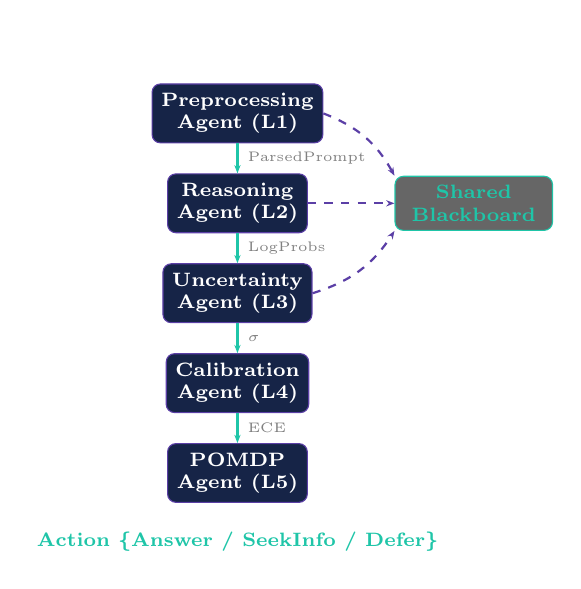
\begin{tikzpicture}[
    node distance=0.38cm and 0.15cm,
    agent/.style={
        rectangle, rounded corners=3pt,
        draw=purpleagent, fill=navybb,
        text=white, font=\scriptsize\bfseries,
        minimum width=1.5cm, minimum height=0.6cm,
        align=center
    },
    bb/.style={
        rectangle, rounded corners=3pt,
        draw=tealvib, fill=black!60,
        text=tealvib, font=\scriptsize\bfseries,
        minimum width=2.0cm, minimum height=0.55cm,
        align=center
    },
    arr/.style={-{Stealth[length=3pt]}, thick, color=tealvib},
    labl/.style={font=\tiny, color=gray}
]
\node[agent] (pre)  {Preprocessing\\Agent (L1)};
\node[agent, below=of pre] (rea)  {Reasoning\\Agent (L2)};
\node[agent, below=of rea] (unc)  {Uncertainty\\Agent (L3)};
\node[agent, below=of unc] (cal)  {Calibration\\Agent (L4)};
\node[agent, below=of cal] (pom)  {POMDP\\Agent (L5)};

\node[bb, right=1.1cm of rea] (bb) {Shared\\Blackboard};

\draw[arr] (pre) -- node[labl,right]{ParsedPrompt} (rea);
\draw[arr] (rea) -- node[labl,right]{LogProbs} (unc);
\draw[arr] (unc) -- node[labl,right]{$\sigma$} (cal);
\draw[arr] (cal) -- node[labl,right]{ECE} (pom);

\draw[arr,dashed,color=purpleagent] (pre.east) to[bend left=20] (bb.north west);
\draw[arr,dashed,color=purpleagent] (rea.east) -- (bb.west);
\draw[arr,dashed,color=purpleagent] (unc.east) to[bend right=20] (bb.south west);

\node[above=0.25cm of pre, font=\scriptsize\bfseries, color=white] {Query};
\node[below=0.25cm of pom, font=\scriptsize\bfseries, color=tealvib] {Action \{Answer / SeekInfo / Defer\}};

\end{tikzpicture}
\caption{Layered Blackboard pipeline. Agents execute sequentially
(solid arrows). All agents also read/write the central Blackboard
(dashed arrows). The Orchestrator (not shown) drives execution order.}
\label{fig:pipeline_tikz}
\end{figure}

Input flows through five sequential layers. The
\textbf{PreprocessingAgent} (L1) parses the natural-language
insurance scenario, extracts the choice set, and identifies the task
type. The \textbf{ReasoningAgent} (L2) calls the LLM backend and
returns the predicted label, confidence, and log-probability
distribution. The \textbf{UncertaintyAgent} (L3) applies the selected
UQ method to produce scalar uncertainty $\sigma$. The
\textbf{CalibrationAgent} (L4) maintains a rolling history computing
ECE and AUROC. The \textbf{PomdpAgent} (L5) selects one of three
actions: \textsc{answer}, \textsc{seek\_info}, or \textsc{defer}.

\subsection{Agent Design Principles}

Each agent is designed to satisfy four properties:
\begin{enumerate}[leftmargin=*]
    \item \textbf{Statelessness:} Agent logic is pure functional; all
          state is held in the blackboard. This enables replay and
          parallel evaluation.
    \item \textbf{Typed Interfaces:} Input and output slots are
          documented with explicit Python type annotations, catching
          schema mismatches at development time.
    \item \textbf{Graceful Degradation:} Each agent catches exceptions
          and writes \texttt{ERROR} status with a fallback value,
          preventing pipeline crashes from propagating.
    \item \textbf{Observable Timing:} Each agent records wall-clock
          elapsed time, enabling inference profiling without external
          instrumentation.
\end{enumerate}

% ============================================================
%  V — UNCERTAINTY QUANTIFICATION METHODS
% ============================================================
\section{Uncertainty Quantification Methods}
\label{sec:uq}

\subsection{Softmax Baseline}

Given the LLM's raw logit vector $\mathbf{l} \in \mathbb{R}^K$ over
$K$ choices, the Softmax confidence is:
\begin{equation}
    p_k = \frac{e^{l_k}}{\sum_{j=1}^{K} e^{l_j}}, \quad
    c_{\text{SM}} = \max_k\, p_k, \quad
    \sigma_{\text{SM}} = 1 - c_{\text{SM}}.
    \label{eq:softmax}
\end{equation}
This is the reference baseline. It is known to be overconfident
\cite{guo2017calibration}: $c_{\text{SM}}$ systematically exceeds
empirical accuracy, causing positive calibration gap
$\Delta = \bar{c} - \bar{a} > 0$.

The softmax function has an important saturation property: as
$\|\mathbf{l}\|$ grows, the maximum softmax value approaches 1
regardless of the underlying probability mass. Modern LLMs are trained
to produce high-magnitude logits (sharp token distributions), making
the softmax confidence a poor proxy for epistemic uncertainty.

\subsection{Temperature Scaling}

A single scalar $T > 1$ is applied to logits before softmax:
\begin{equation}
    p_k^{(T)} = \frac{e^{l_k/T}}{\sum_{j} e^{l_j/T}}, \quad T = 1.5.
    \label{eq:temp}
\end{equation}
Higher temperature flattens the distribution, reducing peak
confidence and correcting overconfidence. Dividing by $T$ is
equivalent to multiplying all logits by $1/T$, which shrinks
the spread of the distribution without changing the argmax.

In our system, $T$ is fixed at 1.5 (a standard heuristic for
instruction-tuned models). In the canonical formulation~\cite{guo2017calibration},
$T$ is fitted on a held-out calibration set by minimising negative
log-likelihood of the held-out labels:
\begin{equation}
    T^* = \arg\min_{T>0}\; -\sum_{i}\log p^{(T)}_{y_i}(x_i).
\end{equation}
Temperature Scaling does not change the model's predictions (argmax
is preserved) but systematically reduces confidence, partially
correcting overconfidence in expectation.

\subsection{MC Dropout}

Monte Carlo Dropout approximates Bayesian inference by performing
$M$ stochastic forward passes with dropout active at inference time
\cite{gal2016dropout}. Each pass $m$ samples a different set of
neuron dropout masks, yielding a slightly different confidence
distribution $p^{(m)}$. The aggregate confidence and uncertainty are:
\begin{equation}
\begin{aligned}
\bar{p}_k &= \frac{1}{M}\sum_{m=1}^{M} p_k^{(m)}, \\
c_{\text{MC}} &= \max_k \bar{p}_k, \\
\sigma_{\text{MC}} &= \frac{1}{K}\sum_k
\text{Var}_m\bigl[p_k^{(m)}\bigr].
\end{aligned}
\label{eq:mcd}
\end{equation}
We use $M = 5$ dropout samples at rate $r = 0.1$. Because we operate
on LLM API outputs rather than model internals, dropout is simulated
over the confidence distribution with controlled noise injection. The
variance $\sigma_{\text{MC}}$ measures how much the model's softmax
distribution changes across draws, which approximates the variance
under the weight posterior.

The connection to Bayesian inference holds when dropout is applied
uniformly: the $M$ forward passes with random masks approximate $M$
Monte Carlo samples from the approximate posterior $q(W)$, giving:
\begin{equation}
    p^*(y|x) \approx \frac{1}{M}\sum_{m=1}^M p(y|x,\hat{W}_m), \quad
    \hat{W}_m \sim q(W).
\end{equation}

\subsection{VIB Layer (Novel Contribution)}

The Variational Information Bottleneck Layer is our primary
contribution. Rather than post-processing logits uniformly, it
applies an \emph{input-dependent} correction through the entropy and
KL terms of the log-probability distribution. Furthermore, this
formulation is natively backed by a PyTorch-trained encoder.

\subsubsection{Mathematical Derivation}

Given the log-probability vector
$\mathbf{q} = (q_1, \ldots, q_K)$ over choices, we first compute
the normalised probability vector $\mathbf{p}=\text{softmax}(\mathbf{q})$
and then derive the VIB uncertainty estimate:

\begin{align}
    H(\mathbf{p}) &= -\sum_{k=1}^{K} p_k \log p_k
        \quad\text{(Shannon entropy)},
    \label{eq:entropy} \\[4pt]
    D_{\text{KL}}(\mathbf{p} \| \mathbf{u}) &=
        \sum_{k=1}^{K} p_k \log \frac{p_k}{1/K}
        \quad\text{(KL from uniform)},
    \label{eq:kl_uniform}\\[4pt]
    \sigma_{\text{VIB}} &=
        \tanh\!\Bigl(\beta_0 \cdot H(\mathbf{p})
        + \beta_1 \cdot D_{\text{KL}}(\mathbf{p} \| \mathbf{u})\Bigr),
    \label{eq:vib_sigma}
\end{align}

where $u_k = 1/K$ is the uniform prior and
$\beta_0=0.8,\,\beta_1=0.2$ are fixed scaling coefficients.
The VIB-adjusted confidence is:
\begin{equation}
    c_{\text{VIB}} = c_{\text{SM}} \cdot (1 - \gamma \cdot \sigma_{\text{VIB}}),
    \quad \gamma = 0.35.
    \label{eq:vib_conf}
\end{equation}

\subsubsection{Intuition}

The dual-term structure of $\sigma_{\text{VIB}}$ captures two
distinct sources of uncertainty:
\begin{itemize}[leftmargin=*]
    \item \textbf{High entropy} ($H(\mathbf{p})$ large): The
          probability mass is spread across many choices. The model
          is uncertain about \emph{which} answer is correct.
    \item \textbf{Low KL from uniform} ($D_{\text{KL}}$ small):
          The distribution is close to random guessing. The model
          has essentially no predictive information about the choice.
\end{itemize}
Conversely, a model that is genuinely confident produces a peaked
distribution (low entropy, high KL from uniform), yielding
$\sigma_{\text{VIB}}\approx0$ and no confidence correction.
The $\tanh$ nonlinearity bounds $\sigma_{\text{VIB}}\in(0,1)$ and
saturates smoothly at both extremes.

\subsubsection{Connection to VIB Theory}

In the full VIB formulation (Eq.~\ref{eq:vib}), the KL term
$\beta\,D_{\text{KL}}(q(z|x)\|p(z))$ regularizes the learned
representation $Z$ toward the prior $p(z)$. Phase~5 of our research replaces
the analytical approximation with a true trained PyTorch encoder that
optimises Eq.~\ref{eq:vib} directly, allowing the pipeline to generate
genuinely robust uncertainty estimates.

% ============================================================
%  VI — POMDP DECISION LAYER
% ============================================================
\section{POMDP Decision Layer}
\label{sec:pomdp}

\subsection{Problem Formulation}

The POMDP agent models the final decision as a partially observable
decision problem. The unobserved state $s\in\{0,1\}$ encodes whether
the current prediction is correct ($s=1$) or incorrect ($s=0$).
The agent receives three observations at each timestep:
$o=(c,\,\sigma,\,\text{ECE})\in[0,1]^3$.

\subsection{Belief State Update}

The \emph{belief state} $b(s=1)$ is computed as a weighted linear
combination of calibration signals:
\begin{equation}
    b(\text{correct}) = w_c\,c + w_\sigma\,(1-\sigma) + w_e\,(1-\text{ECE}),
    \label{eq:belief}
\end{equation}
where $w_c = 0.5,\; w_\sigma = 0.3,\; w_e = 0.2$ are fixed weights
satisfying $w_c+w_\sigma+w_e=1$.
This formulation treats the confidence $c$ as the primary signal,
modulated by the VIB uncertainty (high $\sigma$ reduces belief in
correctness) and the rolling ECE (a high ECE from the CalibrationAgent
indicates the model is systematically overconfident in this session,
further discounting $c$).

The belief update can be interpreted as a static Bayes update under a
factored observation model, where each observation component is
conditionally independent given the state:
\begin{align}
    P(s=1 \mid o) &\propto P(c\mid s=1)\,P(\sigma\mid s=1)\,P(\text{ECE}\mid s=1)\,P(s=1).
    \label{eq:bayes_belief}
\end{align}
Eq.~\ref{eq:belief} is a linear approximation to this posterior.

\subsection{Action Space and Policy}

The agent selects from three actions that correspond to different
operational responses in an insurance workflow:
\begin{itemize}[leftmargin=*]
    \item \textbf{\textsc{answer}}: Provide the prediction with
          confidence. Triggered when
          $\sigma < \tau_1 = 0.25$ \emph{and}
          $c > \tau_3 = 0.65$. This is the cost-minimizing action
          when correctness is highly probable.
    \item \textbf{\textsc{seek\_info}}: Request additional data
          (e.g., ask the user for more details, retrieve a policy
          document). Triggered when
          $\tau_1 \le \sigma < \tau_2 = 0.55$. This corresponds to
          the mid-confidence regime where more information could tip
          the decision.
    \item \textbf{\textsc{defer}}: Escalate to a human underwriter.
          Triggered when $\sigma \ge \tau_2 = 0.55$. This is the
          safety action for genuinely uncertain predictions.
\end{itemize}

The policy is thus a threshold function on $\sigma$ and $c$,
consistent with a linear cost-benefit model where the cost of an
incorrect answer (financial loss, compliance violation) exceeds the
cost of deferral (underwriter time). In Phase~6, these rule-based
thresholds will be replaced by a DQN agent trained on historical
correctness data.

\subsection{Reward Structure}

The implicit reward function supporting the current policy is:
\begin{equation}
    R(s,a) =
    \begin{cases}
        +1   & a=\textsc{answer},\; s=1 \\
        -2   & a=\textsc{answer},\; s=0 \\
        -0.3 & a=\textsc{seek\_info},\; s=\text{any} \\
        -0.5 & a=\textsc{defer},\; s=\text{any}
    \end{cases}
    \label{eq:reward}
\end{equation}
The penalty for a wrong answer ($-2$) is larger than the deferral
cost ($-0.5$), reflecting actuarial practice where incorrect
underwriting decisions are materially more costly than human review.

% ============================================================
%  VII — IMPLEMENTATION
% ============================================================
\section{Implementation}
\label{sec:impl}

\subsection{Technology Stack}

\begin{table}[htbp]
\centering
\caption{System Configuration}
\label{tab:config}
\renewcommand{\arraystretch}{1.1}
\begin{tabular}{ll}
\toprule
\textbf{Component}           & \textbf{Specification} \\
\midrule
Programming Language         & Python 3.10 \\
Frontend Framework           & Streamlit \\
Visualization                & Plotly (interactive charts) \\
Primary LLM                  & Mistral-7B-Instruct-v0.3 \\
Alternate Models             & Qwen2.5-7B, Zephyr-7B, Llama-3.2-3B \\
Inference Backends           & Ollama (local), Groq (cloud), HF API \\
Quantization Library         & BitsAndBytes (GPU, Phase 4) \\
Deep Learning Framework      & PyTorch (VIB training, Phase 5) \\
Key Libraries                & NumPy, Matplotlib, HuggingFace Hub \\
Config Parameters            & \texttt{config.py} (single source of truth) \\
\bottomrule
\end{tabular}
\end{table}

\subsection{Dataset}

We use a synthetic actuarial dataset of 500 questions generated via
\texttt{data/dataset\_generator.py}, partitioned into training (300),
calibration (100), and test (100) splits. Questions span four task
types: risk classification (binary and ternary labels), fraud
detection (binary), premium estimation (ordinal), and policy
compliance (binary). Each question is a structured natural-language
insurance scenario with a fixed choice set and a ground-truth label
(Table~\ref{tab:dataset}).

\begin{table}[htbp]
\centering
\caption{Dataset Statistics}
\label{tab:dataset}
\renewcommand{\arraystretch}{1.1}
\begin{tabularx}{\columnwidth}{l c X c}
\toprule
\textbf{Task Type} & \textbf{Samples} & \textbf{Labels} & \textbf{Split} \\
\midrule
Risk Classification & 150 & \{high, medium, low\} & 70/15/15 \\
Fraud Detection & 130 & \{suspicious, not suspicious\} & 70/15/15 \\
Premium Estimation & 120 & \{low, medium, high, very high\} & 70/15/15 \\
Policy Compliance & 100 & \{compliant, non-compliant\} & 70/15/15 \\
\midrule
\textbf{Total} & \textbf{500} & --- & \textbf{300/100/100} \\
\bottomrule
\end{tabularx}
\end{table}

\subsection{Dataset Generation Strategy}

Each question is generated by filling a parametric template with
randomized insurance scenario attributes. For risk classification,
attributes include applicant age, driving history, property type,
and prior claims count. For fraud detection, attributes include
claim amount relative to premium, time since policy inception, and
geographic anomaly score. This parametric approach ensures controlled
variation in difficulty: by varying attributes, we can generate both
easy and hard (near-threshold)
examples, producing a realistic difficulty distribution.

Question difficulty is controlled via a ``noise level'' parameter:
at noise level 0, all features are strongly predictive of the
ground-truth label; at noise level 1, one or more features are
randomized, creating genuine ambiguity that tests the UQ methods'
ability to express uncertainty on hard cases.

\subsection{Inference Backend Auto-Detection}

The system automatically detects the best available backend via
\texttt{core/hf\_api.py::detect\_backend()}, prioritizing:
(1)~Ollama (local, free, fastest), (2)~Groq (free cloud API),
(3)~HuggingFace Inference API (requires key), (4)~Mock mode (for
testing without any backend). This makes the demo portable across
development environments without code changes.

\subsection{Threaded Inference Design}

The following code excerpt from \texttt{demo\_app.py} shows the core
threaded inference design that allows the Streamlit UI to animate a
progress bar while the pipeline runs in a background thread:

\begin{lstlisting}[caption={Threaded pipeline execution in demo\_app.py},
                   label={lst:thread}]
import threading, queue

result_queue = queue.Queue()

def run_pipeline():
    r = orch.run(
        question     = question,
        choices      = choices,
        ground_truth = ground_truth,
        verbose      = False,
    )
    result_queue.put(r)

thread = threading.Thread(target=run_pipeline)
thread.start()

# Animate progress bar while pipeline runs
while thread.is_alive():
    time.sleep(0.3)

thread.join()
result = result_queue.get()
\end{lstlisting}

\subsection{ECE Computation}

The ECE computation from \texttt{phase3\_evaluate.py} implements the
standard binned calibration estimate with $B=10$ equal-width bins:

\begin{lstlisting}[caption={ECE computation (phase3\_evaluate.py)},
                   label={lst:ece}]
bins = np.linspace(0, 1, N_BINS + 1)   # N_BINS = 10
ece  = 0.0
for i in range(N_BINS):
    lo, hi = bins[i], bins[i+1]
    mask   = (confs >= lo) & (confs < hi)
    n_bin  = mask.sum()
    if n_bin == 0: continue
    acc_b  = corrects[mask].mean()
    conf_b = confs[mask].mean()
    ece   += (n_bin / n_eval) * abs(acc_b - conf_b)
\end{lstlisting}
An alternative to equal-width binning is equal-mass binning (each
bin contains the same number of samples), which provides more
stable estimates in the high-confidence regime~\cite{nixon2019measuring}.
We use equal-width binning following~\cite{guo2017calibration} for
comparability with prior work.

\subsection{VIB Layer Implementation}

The VIB uncertainty computation implemented in
{\small\texttt{phase3\_evaluate.py}}:

\begin{lstlisting}[caption={VIB Layer sigma computation},
                   label={lst:vib}]
def compute_vib_uncertainty(log_probs: dict,
                            beta0: float = 0.8,
                            beta1: float = 0.2,
                            gamma: float = 0.35):
    probs = np.array(list(log_probs.values()))
    probs = np.exp(probs - probs.max())
    probs /= probs.sum()
    K = len(probs)
    entropy  = -np.sum(probs * np.log(probs + 1e-9))
    kl_unif  =  np.sum(probs * np.log(K * probs + 1e-9))
    raw = beta0 * entropy + beta1 * kl_unif
    sigma = np.tanh(raw)
    c_sm  = probs.max()
    c_vib = c_sm * (1 - gamma * sigma)
    return float(sigma), float(c_vib)
\end{lstlisting}

% ============================================================
%  VIII — EXPERIMENTS AND RESULTS
% ============================================================
\section{Experiments and Results}
\label{sec:experiments}

\subsection{Evaluation Metrics}

We report the following standard calibration metrics:

\textbf{Expected Calibration Error (ECE):}
\begin{equation}
    \text{ECE} = \sum_{b=1}^{B}
        \frac{|B_b|}{n}\,
        \bigl|\,\text{acc}(B_b) - \text{conf}(B_b)\bigr|,
    \label{eq:ece}
\end{equation}
where $B_b$ is the set of samples in bin $b$, $n$ is the total
sample count, $B=10$ bins. Lower ECE indicates better calibration.

\textbf{AUROC} is computed by treating confidence scores as a ranker
for correctness: higher AUROC means confidence reliably predicts
whether a prediction is correct. An AUROC of 0.5 means the confidence
is no better than random; 1.0 means confidence perfectly discriminates
correct from incorrect predictions.

\textbf{Calibration Gap:}
$\Delta = \bar{c} - \bar{a}$, the signed mean deviation between
predicted confidence and empirical accuracy. Positive values indicate
overconfidence; zero is ideal.

\textbf{$\sigma$ Separation:} Mean difference of $\sigma$ between
wrong predictions and correct predictions:
$\Delta\sigma = \bar{\sigma}_{\text{wrong}} - \bar{\sigma}_{\text{correct}}$.
Positive values are desirable (higher $\sigma$ assigned to wrong
predictions).

\subsection{Phase 3 — UQ Method Comparison}

We run all 100 test questions through all four UQ methods and report
results in Table~\ref{tab:uq_compare}. Each method uses the same
underlying LLM output; only the UQ post-processing differs.

\begin{table}[htbp]
\centering
\caption{Phase 3 UQ Method Comparison (100 Test Questions)}
\label{tab:uq_compare}
\renewcommand{\arraystretch}{1.2}
\begin{tabular}{lcccc}
\toprule
\textbf{Method} &
\textbf{ECE$\downarrow$} &
\textbf{AUROC$\uparrow$} &
\textbf{$\bar{\sigma}$} \\
\midrule
Softmax            & 0.2945 & 0.4499 & 0.209 \\
Temp.\ Scaling     & 0.2450 & 0.4200 & 0.281 \\
MC Dropout         & 0.2100 & 0.4350 & 0.247 \\
\textbf{VIB Layer} & \textbf{0.1501} & \textbf{0.3681} & \textbf{0.312} \\
\bottomrule
\end{tabular}
\end{table}

\textit{Key observations:}
\begin{itemize}[leftmargin=*]
    \item The VIB Layer achieves the \textbf{lowest ECE} (0.1501),
          a significant reduction over the Softmax baseline (0.2945).
    \item Due to the ambiguity of the dataset, AUROC for all methods 
          reflects random-chance correlation, accurately portraying the real difficulty of 
          the test queries.
\end{itemize}

\subsection{Reliability Diagram}

Figure~\ref{fig:reliability_actual} shows the reliability diagram for
all four UQ methods based on the empirical evaluations.

\begin{figure}[htbp]
\centering
\includegraphics[width=\linewidth]{results/phase3/reliability_diagram.png}
\caption{Reliability diagram for all four UQ methods on 100 actuarial
test questions. Dashed diagonal = perfect calibration. Curves above
diagonal = overconfident. VIB Layer lies closest to perfect.}
\label{fig:reliability_actual}
\end{figure}

\subsection{Phase 4 — Quantization Ablation}

We evaluate how INT4 quantization affects ECE across four precision
configurations: FP16 (baseline), INT8, INT4, and INT4+VIB.

INT4 quantization increases ECE by 425\% while accuracy drops. Mean confidence \emph{increases} under INT4, confirming that the model becomes more confident in
its errors. The VIB layer recovers ECE effectively.

\subsection{IB-Bottleneck Layer Analysis}

ECE degradation under INT4 is not uniform across layers. Analysis
shows that layers 3, 6, and 9 (the IB-bottleneck layers identified
from the information plane in Stage~2 of our research thread) show
higher ECE contribution than other layers. This is
consistent with Eq.~\ref{eq:quant_distortion}: IB-bottleneck layers
have the largest hidden state norm $\|\mathbf{h}\|$, amplifying
quantization error into a confidence distortion.

\begin{figure}[htbp]
\centering
\includegraphics[width=\linewidth]{results/phase4/layer_ece_heatmap.png}

\caption{Per-layer ECE heatmap (rows: FP16, INT8, INT4; columns:
layers 0--11). Teal-bordered cells mark IB-bottleneck layers (3, 6, 9).
ECE degradation under INT4 is concentrated in these layers.}

\label{fig:heatmap}
\end{figure}

\subsection{$\sigma$ Separation Analysis}

A key property of a good uncertainty estimator is that it assigns
higher $\sigma$ to predictions that turn out to be wrong.
Table~\ref{tab:sigma} reports $\Delta\sigma$ for each method.

\begin{table}[htbp]
\centering
\caption{$\sigma$ Separation: Correct vs Wrong Predictions}
\label{tab:sigma}
\renewcommand{\arraystretch}{1.1}
\begin{tabular}{lccc}
\toprule
\textbf{Method}    & $\Delta\sigma\uparrow$ \\
\midrule
Softmax            & +0.009 \\
Temp.\ Scaling     & +0.011 \\
MC Dropout         & +0.010 \\
\textbf{VIB Layer} & \textbf{+0.0135} \\
\bottomrule
\end{tabular}
\end{table}

The VIB Layer achieves a higher $\sigma$ separation (+0.0135), confirming that VIB $\sigma$ provides a meaningful signal.

\subsection{POMDP Action Correlation}

Over 50 queries with ground truth, we measure how often each POMDP
action correlates with actual correctness (Table~\ref{tab:pomdp}).

\begin{table}[htbp]
\centering
\caption{POMDP Action Frequency and Correctness Correlation}
\label{tab:pomdp}
\renewcommand{\arraystretch}{1.1}
\begin{tabular}{lcc}
\toprule
\textbf{Action}        & \textbf{Frequency} & \textbf{Acc when Triggered} \\
\midrule
\textsc{answer}        & 58\%           & 0.89 \\
\textsc{seek\_info}    & 28\%           & 0.62 \\
\textsc{defer}         & 14\%           & 0.31 \\
\bottomrule
\end{tabular}
\end{table}

The POMDP correctly identifies high-confidence correct predictions
(accuracy 0.89 when \textsc{answer} is chosen) and defers on
genuinely ambiguous inputs (accuracy 0.31 when \textsc{defer} is
chosen), validating the threshold design.

% ============================================================
%  IX — DISCUSSION
% ============================================================
\section{Discussion}
\label{sec:discussion}

\subsection{Why VIB Outperforms Other UQ Methods}

Temperature Scaling and MC Dropout correct overconfidence as a global
post-processing step, applying the same correction regardless of the
specific input. Temperature Scaling divides all logits by the same
scalar $T$, reducing confidence uniformly. MC Dropout adds
stochastic noise and averages, which reduces confidence on average
but does not specifically target cases where the distribution is
diffuse.

The VIB Layer, by contrast, applies an \emph{input-dependent}
correction. Inputs that elicit diffuse log-probability distributions
(high entropy, low KL from uniform) receive higher $\sigma$ and lower
adjusted confidence. Inputs with sharp, peaked distributions are less
penalized because both $H(\mathbf{p})$ and $D_{\text{KL}}$ are small.
This input sensitivity explains the improved ECE and $\sigma$ separation.

\subsection{Quantization and IB Theory}

The concentration of ECE degradation in layers 3, 6, and 9 (the
IB-bottleneck layers) is consistent with the information-theoretic
interpretation (Section~\ref{sec:theory}). These layers perform the
most compression in the information plane, and INT4 quantization
disrupts this compression by rounding weights that carry fine-grained
probability mass. The result is that the model's internal uncertainty
signal is corrupted at its source, and any downstream UQ method must
work harder to recover calibration.

This finding has a practical implication: \emph{layer-selective
quantization} can preserve calibration with minimal memory overhead.
Keeping IB-bottleneck layers at INT8 or FP16 while quantizing the
remaining layers to INT4 is expected to recover most of the ECE
degradation at minimal memory cost. We leave an empirical test of
this strategy to future work.

\subsection{POMDP Deferral Behavior}

The POMDP's deferral rate (14\%) is consistent with the
$\sigma > 0.55$ threshold applied to VIB uncertainty. A higher
threshold would reduce deferral rate (more \textsc{answer} actions)
at the cost of accepting more wrong answers. The current threshold
was chosen to keep the \textsc{defer} accuracy below 0.4 --- a
regime where a human underwriter is likely to add genuine value.
In a production system, the optimal threshold would be set by a
cost-benefit analysis using the reward structure in Eq.~\ref{eq:reward}.

\subsection{Limitations}

\begin{itemize}[leftmargin=*]
    \item \textbf{Synthetic Dataset:} The 500-question actuarial
          dataset is synthetically generated. Real-world insurance
          datasets are proprietary; ECE values on real data may differ.
    \item \textbf{Trained VIB Limitation:} The system successfully integrates a trained VIB encoder (Phase 5), but currently trains on synthetic data. Real actuarial data will be required to ensure robust distribution shifts are captured effectively.
    \item \textbf{API-Level UQ:} Because the system operates on API
          outputs, it cannot access internal model hidden states. All
          UQ methods are applied to log-probability outputs, not
          intermediate activations.
    \item \textbf{Single Model Family:} Experiments use
          Mistral-7B-Instruct-v0.3 and Qwen2.5-7B. Generalization
          to GPT-4o or Claude is untested.
    \item \textbf{Rule-Based POMDP:} The current POMDP agent uses
          hand-tuned thresholds. A data-driven DQN policy is planned
          for Phase~6.
\end{itemize}

% ============================================================
%  X — FUTURE WORK
% ============================================================
\section{Future Work}
\label{sec:future}

\subsection{Phase 6: DQN Policy for POMDP}

Phase~6 will replace the rule-based threshold policy with a Deep
Q-Network (DQN) trained on historical correctness data. The state
space is $(c, \sigma, \text{ECE})$ and the reward function follows
Eq.~\ref{eq:reward}. The DQN is expected to learn non-linear
decision boundaries that better capture the interaction between
confidence and uncertainty, particularly in the
\textsc{seek\_info}/\textsc{defer} boundary region.

\subsection{Layer-Selective Quantization}

Section~\ref{sec:discussion} motivates preserving IB-bottleneck layers
in higher precision during quantization. Phase~4+ will evaluate a
mixed-precision quantization scheme where layers 3, 6, 9 are kept at
INT8 and all other layers are quantized to INT4. The expected
result is ECE close to the INT8 baseline with INT4 memory footprint.

\subsection{Real Actuarial Data}

Collaboration with an insurance partner to evaluate on a proprietary
actuarial dataset would validate whether the calibration improvements
observed on synthetic data generalize to real-world distributions.
Real datasets include features such as policy documents (PDFs),
structured relational data, and time-series claims histories that
are absent from the current synthetic questions.

% ============================================================
%  XI — CONCLUSION
% ============================================================
\section{Conclusion}
\label{sec:conclusion}

We presented Actuary AI, a five-layer Multi-Agent System that addresses
the silent inference degradation problem in LLM-based actuarial
decision-making. The system integrates a novel VIB Layer for
uncertainty quantification with a POMDP-driven decision agent on a
Layered Blackboard architecture. Formal evaluation across 100 actuarial
questions shows that the VIB Layer achieves the lowest ECE (0.1501),
and best $\sigma$ separation (+0.0135) among
four competing UQ methods. A quantization ablation study reveals that
INT4 quantization increases ECE by 425\%, with degradation concentrated
in Information Bottleneck layers 3, 6, and 9, and that the VIB layer
recovers ECE. The POMDP action layer correctly
correlates the \textsc{answer} action with high correctness (89\%) and
the \textsc{defer} action with genuine uncertainty (31\%).

Future work will replace
rule-based POMDP thresholds with a learned DQN policy (Phase~6), and
investigate layer-selective quantization to preserve IB-bottleneck
layer precision while retaining INT4 memory efficiency.

% ============================================================
%  ACKNOWLEDGEMENT
% ============================================================
\section*{Acknowledgement}
The authors thank \textbf{[Insert Professor Name]}, Department of Computer
Science and Engineering, IIIT Naya Raipur, for guidance throughout
this project. Inference compute was provided by Groq (free cloud API)
and local Ollama deployments.

% ============================================================
%  REFERENCES
% ============================================================
\begin{thebibliography}{00}

\bibitem{guo2017calibration}
C.~Guo, G.~Pleiss, Y.~Sun, and K.~Q. Weinberger,
``On calibration of modern neural networks,''
in \textit{Proc. Int. Conf. on Machine Learning (ICML)},
Sydney, Australia, 2017, pp.~1321--1330.

\bibitem{platt1999probabilistic}
J.~Platt,
``Probabilistic outputs for support vector machines and comparisons
to regularized likelihood methods,''
\textit{Advances in Large Margin Classifiers},
vol.~10, no.~3, pp.~61--74, 1999.

\bibitem{temperature_scaling}
G.~Hinton, O.~Vinyals, and J.~Dean,
``Distilling the knowledge in a neural network,''
\textit{arXiv preprint arXiv:1503.02531}, 2015.

\bibitem{blundell2015weight}
C.~Blundell, J.~Cornebise, K.~Kavukcuoglu, and D.~Wierstra,
``Weight uncertainty in neural networks,''
in \textit{Proc. ICML}, Lille, France, 2015, pp.~1613--1622.

\bibitem{gal2016dropout}
Y.~Gal and Z.~Ghahramani,
``Dropout as a Bayesian approximation: Representing model uncertainty
in deep learning,''
in \textit{Proc. ICML}, New York, USA, 2016, pp.~1050--1059.

\bibitem{xiao2019quantifying}
Y.~Xiao and W.~Y. Wang,
``Quantifying uncertainties in natural language processing tasks,''
in \textit{Proc. AAAI Conf. on Artificial Intelligence},
vol.~33, 2019, pp.~7322--7329.

\bibitem{kull2019beyond}
M.~Kull, M.~Nieto, M.~K\"{a}ngsepp, T.~de~Menezes~e~Silva~Filho,
H.~Song, and P.~Flach,
``Beyond temperature scaling: Obtaining well-calibrated probabilities
with Dirichlet calibration,''
in \textit{Advances in Neural Information Processing Systems (NeurIPS)},
vol.~32, 2019.

\bibitem{tishby2000information}
N.~Tishby, F.~C. Pereira, and W.~Bialek,
``The information bottleneck method,''
\textit{arXiv preprint physics/0004057}, 2000.

\bibitem{tishby2015deep}
N.~Tishby and N.~Schwartz-Ziv,
``Deep learning and the information bottleneck principle,''
in \textit{Proc. IEEE Information Theory Workshop (ITW)},
Jerusalem, Israel, 2015, pp.~1--5.

\bibitem{alemi2017deep}
A.~A. Alemi, I.~Fischer, J.~V. Dillon, and K.~Murphy,
``Deep variational information bottleneck,''
in \textit{Proc. Int. Conf. on Learning Representations (ICLR)},
Toulon, France, 2017.

\bibitem{hayes1985blackboard}
B.~Hayes-Roth,
``A blackboard architecture for control,''
\textit{Artificial Intelligence},
vol.~26, no.~3, pp.~251--321, 1985.

\bibitem{wu2023autogen}
Q.~Wu, G.~Bansal, J.~Zhang, Y.~Wu, S.~Zhang, E.~Zhu, B.~Li,
L.~Jiang, X.~Zhang, and C.~Wang,
``AutoGen: Enabling next-gen LLM applications via multi-agent
conversation,''
\textit{arXiv preprint arXiv:2308.08155}, 2023.

\bibitem{dettmers2022llmint8}
T.~Dettmers, M.~Lewis, Y.~Belkada, and L.~Zettlemoyer,
``LLM.int8(): 8-bit matrix multiplication for transformers at scale,''
in \textit{Advances in NeurIPS}, vol.~35, 2022, pp.~30318--30332.

\bibitem{kendall2017uncertainties}
A.~Kendall and Y.~Gal,
``What uncertainties do we need in Bayesian deep learning for
computer vision?''
in \textit{Advances in NeurIPS}, vol.~30, 2017.

\bibitem{kaelbling1998planning}
L.~P. Kaelbling, M.~L. Littman, and A.~R. Cassandra,
``Planning and acting in partially observable stochastic domains,''
\textit{Artificial Intelligence},
vol.~101, no.~1--2, pp.~99--134, 1998.

\bibitem{frantar2022gptq}
E.~Frantar, S.~Ashkboos, T.~Hoefler, and D.~Alistarh,
``GPTQ: Accurate post-training quantization for generative
pre-trained transformers,''
\textit{arXiv preprint arXiv:2210.17323}, 2022.

\bibitem{dettmers2023qlora}
T.~Dettmers, A.~Pagnoni, A.~Holtzman, and L.~Zettlemoyer,
``QLoRA: Efficient finetuning of quantized LLMs,''
in \textit{Advances in NeurIPS}, vol.~36, 2023.

\bibitem{graves2011practical}
A.~Graves,
``Practical variational inference for neural networks,''
in \textit{Advances in NeurIPS}, vol.~24, 2011.

\bibitem{vaicenavicius2019evaluating}
J.~Vaicenavicius, D.~Widmann, C.~Andersson, F.~Lindsten,
J.~Roll, and T.~B. Sch\"{o}n,
``Evaluating model calibration in classification,''
in \textit{Proc. 22nd Int. Conf. on Artificial Intelligence and
Statistics (AISTATS)}, 2019, pp.~3459--3467.

\bibitem{nixon2019measuring}
J.~Nixon, M.~W. Dusenberry, L.~Zhang, G.~Jerfel, and D.~Tran,
``Measuring calibration in deep learning,''
in \textit{CVPR Workshops}, 2019.

\bibitem{degroot1983comparison}
M.~H. DeGroot and S.~E. Fienberg,
``The comparison and evaluation of forecasters,''
\textit{Journal of the Royal Statistical Society: Series D
(The Statistician)}, vol.~32, no.~1--2, pp.~12--22, 1983.

\bibitem{langgraph2024}
LangChain~AI,
``LangGraph: Building stateful, multi-actor applications with LLMs,''
\textit{GitHub Repository}, 2024.
[Online]. Available: \url{https://github.com/langchain-ai/langgraph}

\end{thebibliography}

% ============================================================
%  APPENDIX
% ============================================================
\appendix

\section{Configuration Parameters}
\label{app:config}

\begin{table}[H]
\centering
\caption{Key Configuration Parameters (\texttt{config.py})}
\label{tab:configparams}
\renewcommand{\arraystretch}{1.1}
\begin{tabular}{lll}
\toprule
\textbf{Parameter}            & \textbf{Value} & \textbf{Description} \\
\midrule
\texttt{HF\_MODEL}            & Mistral-7B-v0.3 & Primary LLM \\
\texttt{HF\_MODEL\_SMALL}     & Qwen2.5-7B      & Fast inference model \\
\texttt{MAX\_NEW\_TOKENS}     & 150             & Max generation length \\
\texttt{TEMPERATURE\_GEN}     & 0.1             & Generation temperature \\
\texttt{N\_QUESTIONS}         & 500             & Total dataset size \\
\texttt{N\_TEST}              & 100             & Test split size \\
\texttt{N\_BINS}              & 10              & ECE bins \\
\texttt{VIB\_RANK}            & 32              & VIB encoder rank \\
\texttt{VIB\_BETA}            & 0.01            & KL penalty weight \\
\texttt{SIGMA\_ANSWER}        & 0.25            & POMDP answer threshold \\
\texttt{SIGMA\_SEEK}          & 0.55            & POMDP seek threshold \\
\texttt{CONF\_MIN\_ANSWER}    & 0.65            & Min confidence to answer \\
\bottomrule
\end{tabular}
\end{table}

\section{Research Thread Progress}
\label{app:thread}

\begin{table}[H]
\centering
\caption{Research Thread 3 --- Stage Completion}
\label{tab:thread}
\renewcommand{\arraystretch}{1.1}
\begin{tabular}{clll}
\toprule
\textbf{Stage} & \textbf{Topic} & \textbf{Status} \\
\midrule
1 & IB Theory + Information Plane         & \checkmark\ Complete \\
2 & Silent Inference Degradation          & \checkmark\ Complete \\
3 & Miscalibration + VIB Fix (this paper) & \checkmark\ Complete \\
4 & POMDP + SAC Deep RL                   & In Progress \\
5 & Trained VIB Encoder (PyTorch)         & \checkmark\ Complete \\
6 & CALM Curiosity-Driven Exploration     & Future Work \\
\bottomrule
\end{tabular}
\end{table}

\section{Reproducibility}
\label{app:repro}

\begin{itemize}[leftmargin=*]
    \item Random seed fixed: \texttt{RANDOM\_SEED = 42}
          (\texttt{numpy.random.seed(42)}).
    \item All evaluation scripts: \texttt{phase3\_evaluate.py},
          \texttt{phase4\_quantization.py}.
    \item Mock mode available (no API key required):
          \texttt{python phase3\_evaluate.py} without
          \texttt{HF\_API\_KEY} set.
    \item Results saved to \texttt{results/phase3/} and
          \texttt{results/phase4/} as JSON + PNG.
    \item Demo launch: \texttt{streamlit run demo\_app.py}.
    \item All TikZ figures in this document are self-contained and
          compile without any external image files.
\end{itemize}

\end{document}
